\documentclass[10pt]{article}
\usepackage{tikz}
\usetikzlibrary{hobby}

\begin{document}
\begin{center}
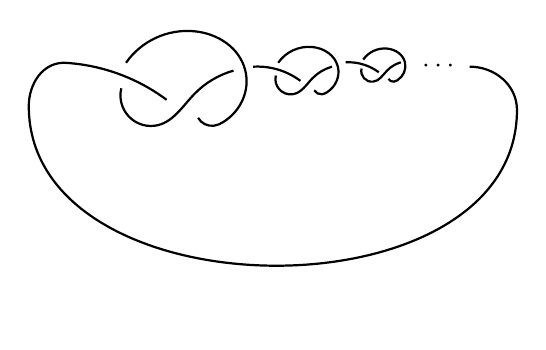
\begin{tikzpicture}[use Hobby shortcut]

    % ENLARGED CURVE 0 (Entry into the first knot)
    \draw[thick] (-0.65, 0.4) .. (-0.38, 0.37) .. (0.65, -0.07);

    % 1. FIRST KNOT
    \draw[thick] (0.075, 0.075) .. (0.5, -0.4) .. (1, 0) .. (1.5, 0.3);
    \draw[thick] (0.135, 0.4) .. (1, 0.8) .. (1.65, 0.3) .. (1.375, -0.35) .. (1.25, -0.4) .. (1.05, -0.3);
    
    % LINE 1 (Connecting 1 and 2)
    \draw[thick] (1.75, 0.35) .. (2, 0.33) .. (2.35, 0.17);
    
    % 2. SECOND KNOT
    \draw[thick] (2.0375, 0.2375) .. (2.25, 0) .. (2.5, 0.2) .. (2.75, 0.35);
    \draw[thick] (2.0675, 0.4) .. (2.5, 0.6) .. (2.825, 0.35) .. (2.6875, 0.025) .. (2.625, 0) .. (2.525, 0.05);
    
    % LINE 2 (Connecting 2 and 3)
    \draw[thick] (2.925, 0.405) .. (3.1, 0.391) .. (3.345, 0.279);
    
    % 3. THIRD KNOT
    \draw[thick] (3.12625, 0.32625) .. (3.275, 0.16) .. (3.45, 0.3) .. (3.625, 0.405);
    \draw[thick] (3.14725, 0.44) .. (3.45, 0.58) .. (3.6775, 0.405) .. (3.58125, 0.1775) .. (3.5375, 0.16) .. (3.4675, 0.195);
    
    % THE ELLIPSIS
    \node at (4.1, 0.35) {$\cdots$};

    % 4. THE U-SHAPED CURVE (Anchored to the new Curve 0)
    \draw[thick] (-0.65, 0.4) 
        to[out=180,in=90] (-1.1, -0.15) 
        to[out=-90,in=-90,looseness=1.1] (5.1, -0.2) 
        to[out=90,in=0] (4.5, 0.35);

\end{tikzpicture}
\end{center}
\end{document}